\chapter{Planteamiento del problema y propuesta}\label{chapter:proposal}

\label{sec:14}

        En esta capitulo se abordarán aspectos referentes a la formulación matemática como un problema de optimización y se identificarán las principales dificultades a enfrentar tanto en el problema de estimación de parámetros como en la propuesta solución. A su vez se propone la arquitectura de agentes.

        \subsection*{ Modelo matemático}

        El problema de estimación de parámetros puede abordarse como un problema de optimización no lineal, en el que la función objetivo se define como la suma de las funciones residuales derivadas de la comparación entre los valores medidos en distintos instantes de tiempo y los valores obtenidos a partir de la solución del sistema de ecuaciones diferenciales ordinarias (EDOs) en función del vector de parámetros. Este modelo de optimización se formula como:

    \begin{equation}
        \min_{\theta} \phi(\theta) = \frac{1}{2} \sum_{i=1}^{M} (y(t_i, \theta) - \tilde{y}_i)^T (y(t_i,    \theta) - \tilde{y}_i)
    \end{equation}

    s.a.:


        \begin{center}

        $\dot{y}(t, \theta) = f(y(t, \theta), t, \theta)$ \\
        $y(0) = y_0$ \\
        $0 \leq t \leq T$ \\
        $y \in \mathbb{R}^n, \quad \theta \in \mathbb{R}^k, \quad f : \mathbb{R}^n \times \mathbb{R}^k \times [0, T] \rightarrow \mathbb{R}^n$

        \end{center}

    Donde:
    \begin{itemize}
        \item $\theta$: es el vector de parámetros a estimar que permite ajustar el modelo.
        \item $y(t_i, \theta)$: son los valores de las variables, obtenidos mediante la solución numérica del sistema de EDOs.
        \item $\tilde{y}_i$: son los valores observados de la función $y(t_i, \theta)$ en diferentes momentos $t_i$ $(i = 1, ..., M)$.
        \item $y(0)$: solución inicial para el sistema de EDOs.
    \end{itemize}

    La evaluación de la función objetivo en este contexto está intrínsecamente ligada a la solución numérica del sistema de ecuaciones diferenciales ordinarias (EDOs). Este problema se conoce como Problema de Valor Inicial. Este enfoque implica determinar las condiciones iniciales que permiten resolver las EDOs, garantizando así que la solución obtenida sea válida y útil para la estimación de parámetros en el modelo propuesto.

        La estimación de parámetros enfrenta desafíos significativos, que pueden clasificarse en dos categorías principales: incertidumbre en los datos y complejidad computacional. A continuación, se listan estas dificultades. \\


        \begin{center}
            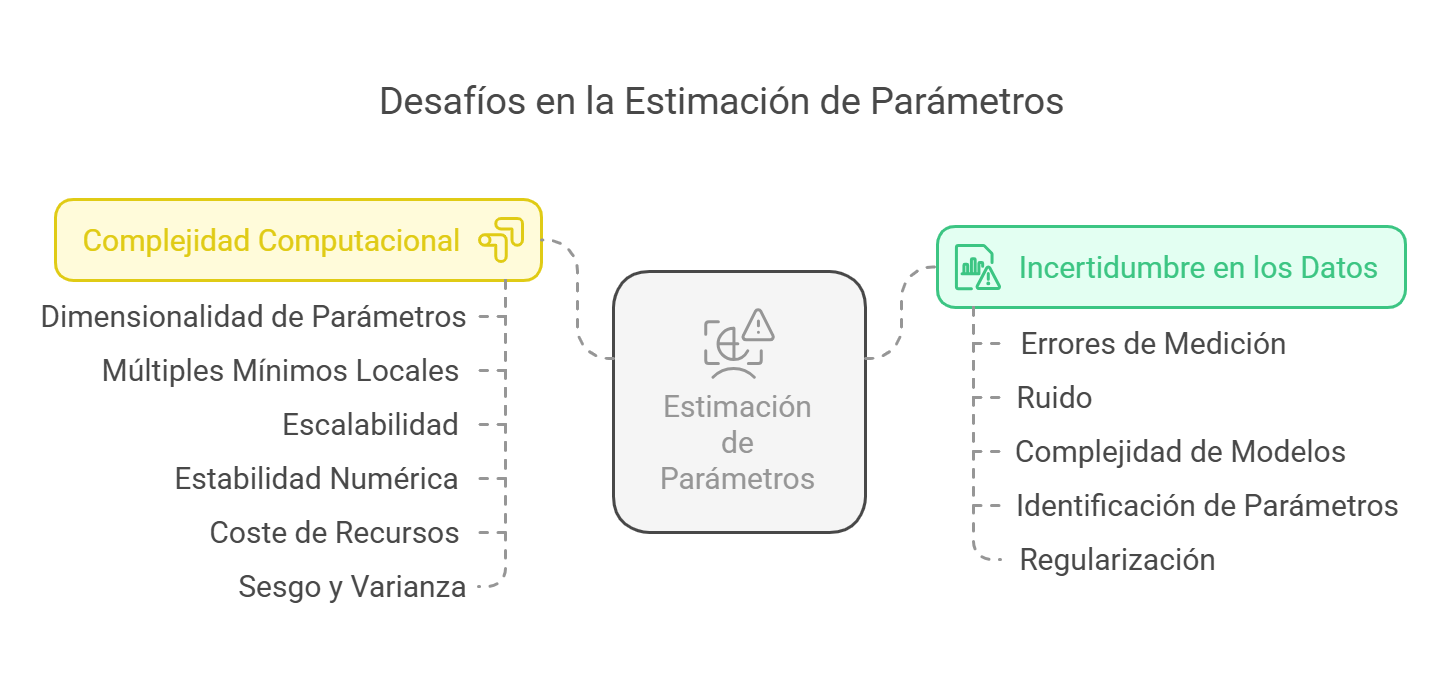
\includegraphics[width=1\textwidth]{images/visual-selection.png}
            \begin{center}
                fig 1. Desafíos en la Estimación de Parámetros
            \end{center}
    \end{center}

        En este caso usaremos intervalos para mitigar errores en mediciones, sin embargo, presupone un desafío estimar el intervalo donde se encuentra el parámetro con un error $w(I) < \epsilon$  donde $I$ es un intervalo.\\



        \subsection*{ Problemas a resolver para conseguir una arquitectura de agentes cooperativos que integran análisis de intervalos }

        La arquitectura propuesta debe lidiar con las anteriores dificultades, los agentes deben ser capaces de actuar en un ambiente dinámico y estimar el intervalo de salida más efectivo, a su vez deben activarse ante los estímulos correctos y saber ignorar otros que ocurren en el ambiente. Los agentes deben ser capaces de cooperar entre sí y saber cuándo parar de iterar entre ellos para devolver el resultado que minimice el valor esperado. A continuación, se listan varios puntos que detallan los desafíos de la arquitectura.\\
        \begin{itemize}

            \item Modificar el espacio de llegada de cada agente para conseguir un espacio de salida
            \item Saber cómo parar dado que los agentes pueden crear ciclos de iteración entre ellos.
            \item Cada agente debe saber en cada iteración con qué agentes interactuar.
            \item Los agentes deben saber qué hacer cuando cometen errores, es decir, el error debe minimizarse en el tiempo.\\

        \end{itemize}

\label{sec:15}

    \subsection*{ Análisis de restricciones de la arquitectura de agentes}

        Para atacar el primer punto que se encuentra en las dificultades de la arquitectura en el capítulo anterior se tiene que definir el espacio de llegada que recibe el agente y el espacio de salida. Para ellos se hacen las siguientes consideraciones.\\

        Cada agente en cada iteración tiene un conjunto de precondiciones que lo activan, es decir, denotamos a $P$ como el conjunto de precondiciones y se define como $P=[ p_0,p_1,...,p_n]$ donde $p_i$ es una precondición que puede ser verdadera o falsa. $P \iff p_0 \land p_1 \land...\land p_n$. En este caso se considera verdadera que la precondición $p_i$ adquiera un valor. Por ejemplo, si el universo de precondiciones es $U=[p_0,p_1,...,p_n]$ y $P=[p_0,p_1,...,p_k]$ siendo $k<n$ entonces las precondiciones $[p_{K+1},...,p_n]$ son falsas para el agente. \\

        Se define el conjunto de acciones que puede tomar el agente donde cada acción puede ser refinada a un conjunto potencialmente infinito de acciones. Es decir, sea $F(P,X)=Z$, entonces $Z$ es una acción a tomar por el agente, donde $P$ son las precondiciones y $X$ los valores de entrada del agente \\

        En el segundo punto se requiere que los agentes deben saber parar las iteraciones puesto que pueden darse ciclos, se toman cotas superiores de iteración. Si los agentes no paran llegado este número, se devuelve el resultado generado hasta ese momento. Este método es robusto para detener las iteraciones, más adelante se verá un método iterativo que asegura la convergencia de las iteraciones. \\

        Para atacar el punto tres es necesario modelar la red de arcos entre agentes. Sea $M$ el número de agentes, si dos agentes $A$ y $B$ están conectados, entonces ocurren una de las siguientes condiciones:

        \begin{itemize}
            \item $A\rightarrow B$, $A$ 'escucha' de $B$
            \item  $B \rightarrow A$, $B$ 'escucha' de $A$
        \end{itemize}

        Si $A$ escucha de $P^n=[A_0^n,A_1^n,...,A_k^n]$ entonces las precondiciones de $A$ son $P=\lceil p_0 - \frac{1}{2} \rceil \lor \lceil p_1 - \frac{1}{2} \rceil \lor \dots \lor \lceil p_n - \frac{1}{2} \rceil$ donde: 
        $p_i=A_k$. Las expresiones $A_0^n,A_1^n,A_k^n$ se refieren al valor de las ponderaciones de los arcos $A_0,A_1,\dots,A_n$ en la iteración $k$. Es preciso notar que $p_i \in [0,1]$ \\

        Como última observación se dice que si en un instante $k$ no hay arcos entre agentes, entonces hemos convergido a un resultado final.

    \subsection*{Arquitectura de Agentes Cooperativos}

        Antes de saltar sobre los detalles de la arquitectura es necesario precisar que la arquitectura propuesta se basa en una red de agentes donde cada uno tiene una funcionalidad específica y se entrena para mejorar sus resultados. Notar que este entrenamiento es supervisado. \\

        La arquitecta está divida en cuatro agentes: los agentes de entrada, los agentes de salida, agente coordinador de acciones y el agente corrector de acciones. Lo siguiente asume que la función tiene la forma $R^n \xrightarrow{f} R^m$. \\

        Agentes de entrada: Estos agentes reciben una entrada $X$ y devuelve un valor $y$, es decir sea $FoT$ la función del agente $i$, entonces el agente recibe $(P,X)$ donde $P$ son las precondiciones, $X$ los valores de entrada y
        $T(P,X)=p_0x_0 + p_1x_1 +...+p_nx_n$ siendo $n$ el número de agentes, luego envía su resultado al puerto de salida para que otro agente la escuche. Estos agentes no son los responsables al menos de forma directa de la salida de la red.\\

        Agentes de salida: Existe un agente de salida por cada parámetro de salida estos agentes son los responsables de escuchar de los agentes de entrada y devolver la salida.
        Un punto importante es que existen tantos agentes de salida como parámetros de salida se definen. Al igual que los agentes de entrada estos implementan una función $FoT$ 
        que recibe la tupla $(P,X)$ y devuelve un valor $Y$ que es donde se espera que este la respuesta. Estos agentes se determinan al inicio del entrenamiento.

        Un punto importante a destacar es que la función de $F$ de ambos agentes, es su función característica, es decir, una función que solo implementan ellos y además se exige que sea inversible.

        Agente coordinador: Este agente se encarga de resolver en cada $k$-iteración las arcos entre agentes. Este agente recibe como entrada, la entrada a la red 
        y devuelve los arcos entre agentes. Si este agente no define arcos entre agentes, el resultado de la red está en el valor de los agentes de salida definidos. Este agente se entrena 
        a partir de los errores cometidos por sus arcos estimados. Este agente puede ser un regresor que sea capaz de recibir una entrada $m$ de parámetros y devolver
         un vector $V$ donde $|V|=(|$ Agentes de Entrada $| + |$ Agente de salida $|)(|$ Agentes de Entrada $| + |$ Agente de salida $| - 1)$ y además $v_i \in [0,1]$.
          El vector $V$ codifica la matriz $W$ de agentes donde la componente $w_{ij}$ refleja el peso de los arco entre el agente $i$ y el agente $j$, este valor es una 
          medida de cuando influye en el agente $i$ las decisiones del agente $j$.\\

        \textbf{Definición de generación}: Dada una lista $L$ de pares $(x,y)$ se define como generación al $g$-ésimo par $(x,y)$. \\

        Por cada generación la red interactúa para dado un vector $X$, devuelva un vector $Y$.\\

        Uso de intervalos \hyperref[sec:24][14]: Se usan intervalos para computar el rango de valores más probables en cada interacción de los agentes. Como hemos dicho anteriormente, cada agente recibe una combinación lineal
        que corresponde a la salida de agentes a los que está conectado, es decir $X=[X_0,X_1,...,X_n]$ donde cada $X_i$ es un intervalo. \\

        Regla de la ecuación lineal \hyperref[sec:25][15]:

                $$\frac{\left\langle \sum_{i=1}^{n} a_i x_i = b ; \; x_1 \in D_1, \ldots, x_n \in D_n \right\rangle}
                {\left\langle \sum_{i=1}^{n} a_i x_i = b ; \; x_1 \in D'_1, \ldots, x_n \in D'_n \right\rangle}$$

            dónde $i \neq j$

            \[ D'_i := D_i, \]

            \[ D'_j := D_j \cap \frac{b - \sum_{i \in [1..n] - \{j\}} int(a_i \cdot D_i)}{a_j}. \]

            Esta regla es aplicada a los números enteros, sin embargo, se puede extender a los números reales, dado que un resultado de la aritmética de intervalos la cual se define en reales.\\

        Agente corrector: Este agente corrige los arcos generadas por el agente coordinador y las envía al agente coordinador para que este las tome en cuenta en su próxima generación. Recibe como entrada el estado de los agentes de entrada y salida y los arcos entre estos. Este agente actúa una vez que la red pare sus iteraciones. \\

        Sea $V$ la salida del agente coordinador que codifica la matriz $W$, se calcula la diferencia entre el intervalo esperado y el intervalo de salida de los agentes de salida.
        Como se quiere que la red resuelva el problema en la menor cantidad de interacciones, comenzamos desde la iteración 1 a buscar qué arcos habrían dado la
        respuesta correcta. Por cada agente de salida buscamos qué o cuales agentes de entrada darian la respuesta correcta.  \\

        Se propone encontrar un grafo $G$ tal que $\underset{G}{\min}(||F(X)-Y||)$. Como se conoce la respuesta correcta $Y$, entonces la componente $y_i \in Y$ debería ser el valor de salida del agente de salida $i$-ésimo, para determinar cuáles debieron ser los valores de entrada, hacemos $r=f^{-1}(y_i)$ y $r'=T(X,P)=p_0X_0 + p_1X_1 +...+p_kX_k$ como se conocen los valores de $X$ y de $P$
        entonces el agente corrector debe buscar en la red qué agentes minimizarían $T=[|r-r'|,|r-r'|]$. Tenemos entonces dos posibles casos: \\

        Caso 1: $[|r-r'|,|r-r'|] > \sum_{i=k+1}^{n} a_iX_i$ siendo $a_i=1$, $n$ el número de agentes de salida más agentes de entrada y el intervalo de $[k+1,n]$ los agentes
        que no forman parte de la salida. Aquí basta con conectar de forma sucesiva los agentes $X_{k+j}$ con $j=1,2,..n$ hasta que $[|r-r'|,|r-r'|] \leqslant \sum_{i=k+1}^{k+j} a_iX_i$ si la relación es de igualdad, hemos encontrado los arcos,
         si es menor estricto, nos lleva al caso 2.\\

        Caso 2: Si $[|r-r'|,|r-r'|] \leqslant \sum_{i=k+1}^{k+j} a_iX_i$ siendo $a_i=1$, entonces solo despejamos uno de los agentes para encontrar el peso que iguala la ecuación
        es decir: $D(a_{k+j}) \cap \frac{[|r-r'|,|r-r'|] - \sum_{k+1}^{k+j-1} X_i}{|X_{k+j}|}$.\\

        Una vez concluidos los hallazgos en la primera iteración, esta es enviada al agente coordinador, para que se ajuste dada la tupla $(X,Y)$ siendo
        $X$ los valores de entrada a la red y $Y$ los arcos de salida, concluido esto, el agente corrector pasa a la iteración 2 y comienza nuevamente la búsqueda de el arco ideal. Una vez concluido este proceso
        el agente corrector hace el mismo proceso, pero esta vez asumiendo que la salida de la primera interacción es la entrada de la segunda iteración, es decir $\underset{X}{\min}([|r-r'|,|r-r'|])$ donde $X$ es el vector estado de la red luego de minimizar $[|r-r'|,|r-r'|]$.
        De igual forma la red continua con la siguiente iteración hasta terminar con la cola de iteraciones de la generación. Luego de pasar por todo este proceso la red comienza nuevamente con la siguiente generación de datos. \\

        Se itera dos veces sobre la pila de iteraciones porque es necesario entrenar el agente coordinador y para ello se requiere la mayor cantidad de datos posibles. Pues el primer entrenamiento se hace para rectificar los arcos erróneos, y el siguiente para aprender la respuesta correcta.
        Es importante destacar que existen infinitos grafos correctos, es por esto que el agente coordinador tiene tal comportamiento greedy.

        \subsection*{Ciclos de iteración}

         Al inicializarse la red, esta recibe un vector de entrada, luego el agente coordinador determina los agentes de salida y los arcos entre agentes. Notar que todos los agentes excepto los agentes que se determinan que son entrada, son de salida, es decir, todos los agentes de entrada reciben el vector de entrada en el primer ciclo de interacción. Para la $k$-iteración el agente coordinador cambia las arcos de los agentes y el agente $i$-ésimo recibe ahora los valores de salida de sus nuevos arcos en la $(k-1)$ iteración. Los agentes de entrada y salida comienzan a iterar hasta detenerse o hasta llegar a una cota máxima de interactividad, terminado este paso, el agente corrector corrige los arcos basado en el error cometido por la red y las envía al agente coordinador, terminado esto, estamos listo para pasar con la siguiente iteración. \\

        Notar que estos agentes paran las iteraciones si y solo si no se activa ninguna precondición de los agentes que esto a su vez conicide con que no existan arcos entre agentes. En la siguiente figura 1 se ilustra el proceso descrito: \\


        \begin{center}
                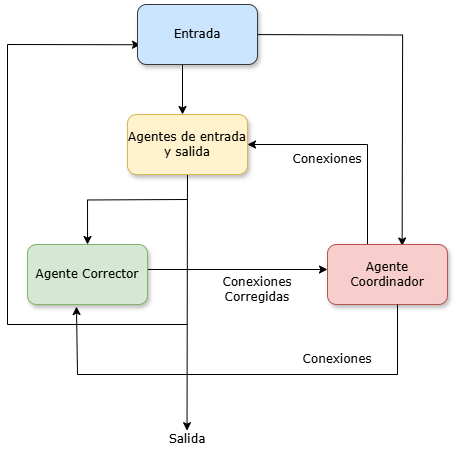
\includegraphics[width=0.6\textwidth]{images/AgentArchitecture.drawio.png}
                \begin{center}
                    fig.2 Flujo de trabajo entre los agentes
                \end{center}
        \end{center}